% This must be in the first 5 lines to tell arXiv to use pdfLaTeX, which is strongly recommended.
\pdfoutput=1
% In particular, the hyperref package requires pdfLaTeX in order to break URLs across lines.

\documentclass[11pt]{article}
\usepackage{graphicx}
\usepackage{wrapfig}
\usepackage{amsmath}

% Remove the "review" option to generate the final version.
\usepackage[]{ACL2023}

% Standard package includes
\usepackage{times}
\usepackage{latexsym}

% For proper rendering and hyphenation of words containing Latin characters (including in bib files)
\usepackage[T1]{fontenc}
% For Vietnamese characters
% \usepackage[T5]{fontenc}
% See https://www.latex-project.org/help/documentation/encguide.pdf for other character sets

% This assumes your files are encoded as UTF8
\usepackage[utf8]{inputenc}

% This is not strictly necessary, and may be commented out.
% However, it will improve the layout of the manuscript,
% and will typically save some space.
\usepackage{microtype}

% This is also not strictly necessary, and may be commented out.
% However, it will improve the aesthetics of text in
% the typewriter font.
\usepackage{inconsolata}

\title{Assessing the Impact Score of Scientific Publications through the Analysis of Abstracts and their Metadata}

\author{Artem Lebedev\\
  UC Berkeley / Berkeley, CA \\
  \texttt{artem.lebedev@berkeley.edu} \\\And
 Farouk Ghandour \\
  UC Berkeley / Berkeley, CA \\
  \texttt{fghandour18@berkeley.edu} \\}

\begin{document}
\maketitle

\begin{abstract}
An impact score of the academic paper is a metric critically important for a scientist's career and attraction of funding for future research. The ability to predict the potential score of a paper could help scientists adjust their presentation strategy to achieve maximum impact. Natural language processing (NLP) is a logical tool to examine what leads to a scientific article's strong impact score because it allows one to analyze an article’s content numerically. In this paper we investigate if the content of the abstract matters for the selection of the journal, or meta-factors, such as author address and number of co-authors are sufficient to select the bset possible journal for submission.\footnote{The code and data available on \href{https://github.com/ArtemChemist/w266_project}{GitHub} and \href{https://drive.google.com/drive/folders/1OkSzswtFvqA6_FD35vvSCU31kSd1ECA2?usp=drive_link}{GDrive}.}
\end{abstract}

\section{Introduction}
A measurement of the academic paper's impact is critically important for a scientist's career and attraction of funding for future research. The ability to predict the paper's significance could help researchers adjust their presentation strategy to achieve maximum visibility. Our team aims to elucidate the factors that drive acceptance in high-impact journals.

Our hypothesis is that variation in the impact of an academic paper can be mostly explained by the metadata of the paper: country of origin, number of authors, length of the paper etc. The metrics of impact that is the most amenable for the quantitative analysis is Journal Impact Factor (JIF), wich is, roughly, the average number of times papers in the journals are cited in the works of others.   

We selected Pearson's correlation coefficient between the predicted impact and observed impact as the metric to evaluate and compare models. We will assume that we failed to reject null hypothesis if observed-predicted correlation of the model including text data and metadata is not significantly larger than correlation achieved with the same model lacking text data (Eq.~\ref{eq:hypothesis}).
\begin{equation}\label{eq:hypothesis}
	\begin{cases}
		H_{0}: (r_{w\ text} - r_{only\ metadata}) \leq 0 \\
		H_{A}: (r_{w\ text} - r_{only\ metadata}) > 0\\
	\end{cases}       
\end{equation}
In the social science context correlation coefficient above 0.5 is generally considered moderately positive\citep{KahnemanDaniel2021N:af}. Following this convention, we will consider our findings to be practically significant only if at least one coefficient exceeds 0.5. If both coefficients are below 0.5, it is likely that our research question can not be answered with this data set and our approach. 

\section{Background}
% Not done. Supppoesed to describe motivation for the work.
A few attempts have been made to address this issue, demonstrating modest but encouraging success. \citep{Macri2023-tr, Alohali2022-no, 10.1162/qss_a_00258, doi:10.1152/japplphysiol.00489.2020} The most sophisticated model utilized BERT context-aware encoding of the abstract to produce embedding that were then classified using  SVM, logistic regression or XGBoost to predict the impact factor quintile. This approach demonstrated prediction accuracy of approx. 75%.

\section{Data}
We will rely on the data extracted from the Web of Science, a platform that provides access to citation metrics for the majority of life science publications. The platform allows downloading csv files with the article abstract along with the ISSN identifier of the journal and other metadata. To reduce variability unrelated to the research question we will focus on a narrow field of radioligand therapy and select only original peer-reviewed articles published in English between 2000 and 2022. JIFs are available from Claritive Analytics “Journal Impact Factor Report” and contain the journal ISSN as well as the impact factor, by year. Merging these two datasets on ISSN we achieve our raw dateset, containing approximately 4500 records.

Since our aim is to support researcher decision on publication strategy, we focus on the features that are available to the paper authors at the time of submission: 'Year Published', 'Authors', 'Document Title', 'Author Keywords', 'Abstract', 'Author Address', 'Funding Agency and Grant Number', 'Cited Reference Count', 'Page Count'. Using author identities as features would result in very sparse set of categorical variables, therefore we reduced the author information to just the number of authors and the author address to just the country. We also reduced the funding information to a binary variable funded/not-funded.

'Abstract' is the most important and relevant feature of the paper. Together with the title and author's keywords it represents condensed meaning of the paper. Full text of the paper would have been a lot more information reach, but would also require significantly more computational resources. 

Figure~\ref{fig:paiplot} shows the distribution and correlation matrix for the main quantitative variables available in the metadata. Figure~\ref{fig:countries} demonstrates distribution of the papers by the country of author's origin and the country where the paper was published. Domination of the USA is not surprising, given the preference for English language. Notably, most papers from non-English speaking authors, which is likely not reflected in the training of BERT model that we will be using later.
\begin{figure}
	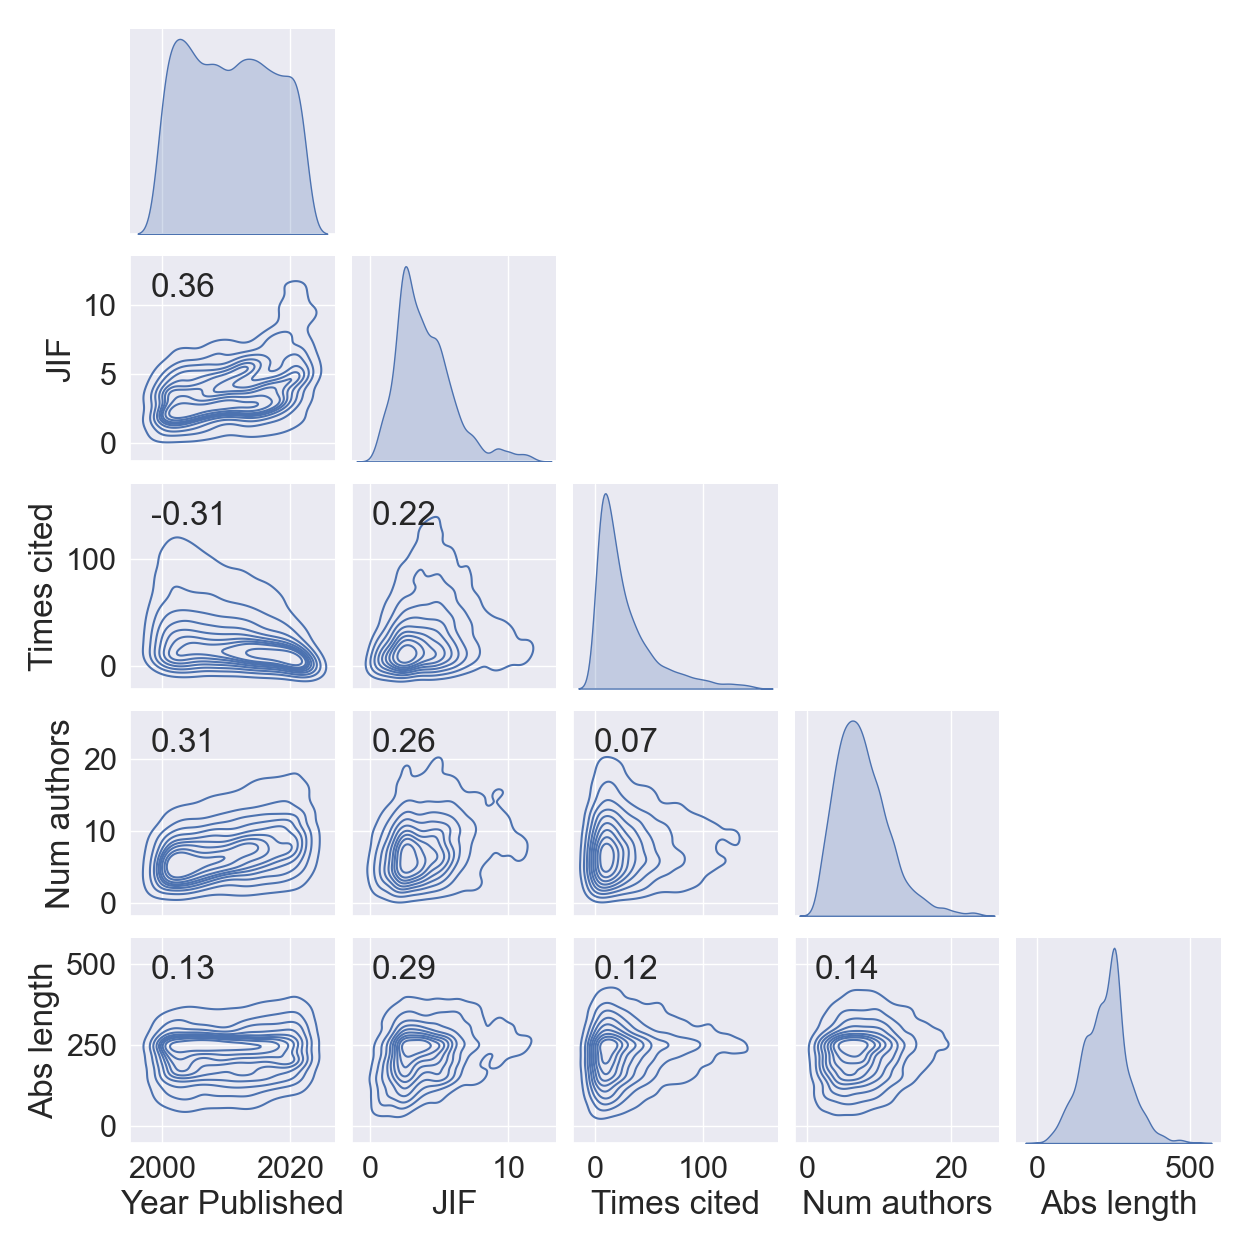
\includegraphics[width= \columnwidth]{./Images/Pairplot.png}
	\caption{Correlation plot of main numerical features}
	\label{fig:paiplot}
\end{figure}

\begin{figure}
	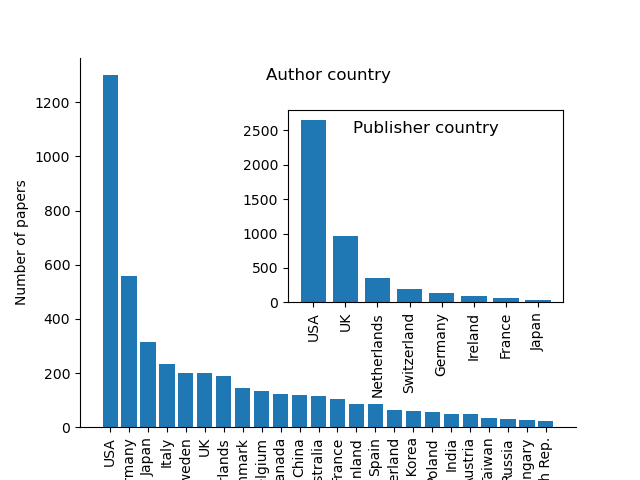
\includegraphics[width= \columnwidth]{./Images/Countries.png}
	\caption{Countries of authors and publishers}
	\label{fig:countries}
\end{figure}

\section{Methods}
We will use regression models based on neural networks to predict the impact of the publications. To evaluate the importance of text data, we will compare predictive power of the model that includes text data vs the model that is based solely on metadata. We will reject null hypothesis if the addition of text data to the model significantly increase the Pearson's correlation coefficient between observed and predicted impact values.

Features selected after EDA fall into three general categories: numerical features, categorical features and text. While numerical features can be included into the model as-is, categorical variables and text need to be transformed before they become inputs into neural network. One-hot-encoded representation is a common way to transform categorical variables, but it lacks the ability to capture patterns present in the data. For instance, papers originating from Canada are likely similar to ones written in the USA, but very different from papers submitted from China. To preserve these patterns, we have chosen to use learned embedding representation of the categorical variables \citep{DBLP:journals/corr/GuoB16}.

Transformation of text into contextually-aware embedding is commonly achieved using BERT \citep{DBLP:journals/corr/abs-1810-04805}. sciBERT, a similar model trained on the large corpus of medical and scientific literature, was recently presented \citep{DBLP:journals/corr/abs-1903-10676} and we plan to compare these two models. Both variants of BERT yield several vectors that can represent the text: pooled vector, cls vector or a set of vectors for each input token. 

The exact way representations of numerical, categorical and text data are combined will be investigated. For the baseline model we concatenated all three vectors and used them as input into a linear regression. In the future we plan to also subdivide the abstract into individual sentences and use cls tokens for more fine-grained text representation. We also plan to use the 2D-representation of text based on the individual word embedding (or sentence-level cls tokens) and process it with convolutional  neural network. Other combinations of the sentence-level and abstract-level embeddings can be used as well \citep{hs2022}. It is also intriguing to use individual embeddings of the keywords, because they were selected by the authors as the most representative of the paper.

\section{Results and discussion}
We investigated influence of a few model architecture choices on the final model performance. Any model would require a dense layer prior to regression output layer and we investigated how the number of dense layers affected performance. We used cls token generated by standard uncased BERT and added no dense layers, one or two dense layers on top of the 768-dimensional vector. All dense layers had 768 neurons. Correlation between predicted and observed JIFs improved upon addition of the first layer (r = 0.51 vs 0.54 p = 8e-07 assuming dependent samples), but did not improve with addition of the second dense layer (r = 0.544 vs 0.538 p = 0.18). However,  Figure~\ref{fig:dense} shows that the histograms of predicted and observed JIFs matched a lot closer for the model with 2 dense layers. To avoid overfitting we did not increase the number of layers further and used 2 dense layers in all subsequent experiments.

\begin{figure}
	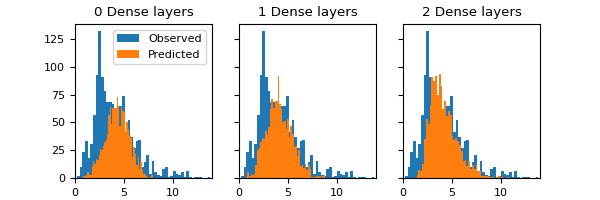
\includegraphics[width= \columnwidth]{./Images/Dense layers.png}
	\caption{Observed-Predicted for different number of dense layers.}
	\label{fig:dense}
\end{figure}

Replacing standard BERT with sciBERT, a model trained on scientific text, we further improved the result (r = 0.54 vs 0.61 p = 1e-08). 

For the baseline model we built a two regression models. One based on metadata only was based on numerical features concatenated with learned embedings for each of the categorical features. The resulting vector was fed directly into the dense output layer with one element and linear activation. Interestingly, adding additional dense layers before the out layer did not improve performance of this baseline model. The model including text data had identical architecture, but also included cls token of uncased BERT output from the abstract. Figure~\ref{fig:meta_no_meta} shows correlation plots obtained for two models. Observed-predicted Pearson's correlation using metadata alone was 0.38, and adding BERT's cls token improved it to 0.47 (p = 0.0034 after Fisher's transformation, one-tailed, assuming independent samples). 
\begin{figure}
	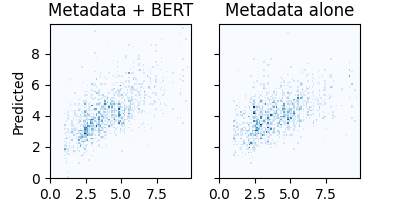
\includegraphics[width= \columnwidth]{./Images/Metadata w BERT.png}
	\caption{Observed-Predicted for models w metadata.}
	\label{fig:meta_no_meta}
\end{figure}

While the improvement from adding text data was statistically significant, neither model crossed our pre-determined threshold of r = 0.5, casting doubts on the predictive power of this approach. To improve the correlation we experimented with model based on BERT token alone. Surprisingly, just cls token from the BERT transformation of abstract, coupled with a dense layer and a regression layer yielded r=0.50 and switching to sciBERT improved it even further, up to 0.56 (p = 0.021). Figure~\ref{fig:BERT_vs_sciBERT} illustrates this experiment. Notably, the learning curves indicated significant over-fitting despite aggressive 0.3 dropout.

\begin{figure}
	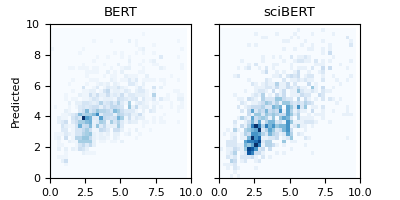
\includegraphics[width= \columnwidth]{./Images/BERT vs sciBERT.png}
	\caption{Observed-Predicted for two BERT models.}
	\label{fig:BERT_vs_sciBERT}
\end{figure}

\section{Conclusions and Next Steps}
Our preliminary experiments strongly support rejection of null hypothesis, but practical usability of the predictions from our model is still in question.

To improve observed-predicted correlation we plan to investigate using sentence-level cls-tokens as well as full set of word embeddings, possibly in combination with CNN architecture. To combat over fitting we plan to enrich data set by adding concatenating titles to abstracts. As a long-shot experiment we also plan to augment data with synthetic abstracts compiled from individual sentences of papers published in the same journal in the same year.

Target variable transformation might be beneficial as well. Presently we use linear regression, which might produce negative values. By replacing JIF with JIF rank calculated on the training data set and using sigmoid activation on the output layer, we might achieve improved model performance. 

% Entries for the entire Anthology, followed by custom entries
\bibliography{custom}
\bibliographystyle{acl_natbib}

\end{document}
